% Chapter Template

\chapter{FDTD - One-Dimensional Scenario} % Main chapter title

\label{Chapter2} % Change X to a consecutive number; for referencing this chapter elsewhere, use \ref{ChapterX}

In this chapter, we will go more in depth into developing an application that can generate electromagnetic data in a one-dimensional domain. In the previous chapter, we mentioned a series of steps to implement FDTD, and that a part of them depend on the particular implementation. A keen eye will notice moving forward, that while the code will not change too much, each implementation deserves a different approach in the theoretical sense.

%----------------------------------------------------------------------------------------
%	SECTION 1
%----------------------------------------------------------------------------------------

\section{1D Discretization}

In the previous chapter, we ended up with the equations \ref{eqn:electricUpdateIntegral} and \ref{eqn:magneticUpdateIntegral}. They will now be used to do a FDTD discretization for the one-dimensional electromagnetic wave scenario. At the end of this section, we will have the update equations that we will use in our loops. Before moving on, we must first briefly discuss tranverse modes. A tranverse mode is the type of pattern that an electromagnetic field, which is perpendicular with respect to the direction of the wave's propagation, has. For electromagnetic waves, the most relevant modes are TE (Tranverse Electric) and TM (Tranverse Magnetic). In our scenario, we will be using TE mode for discretization.

%-----------------------------------
%	SUBSECTION 1
%-----------------------------------
\subsection{Spatial and Temporal Shift}

The first step of the FDTD discretization is a shift in spacetime of the electric and magnetic fields. This spatial shift is shown in Figure \ref{fig:fdtd1dDiscretized}.

\begin{figure}
	\centering
	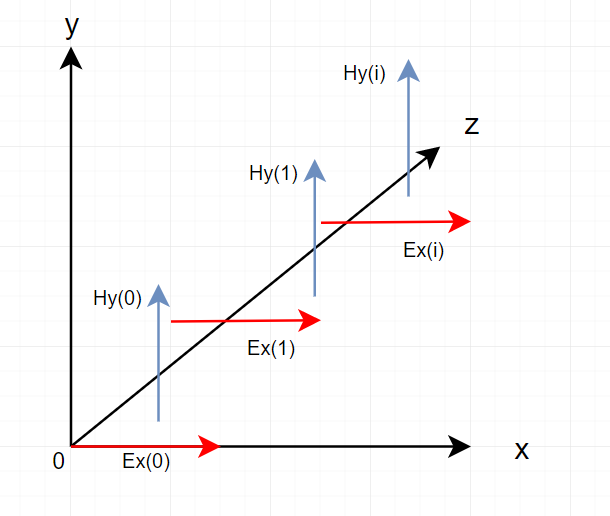
\includegraphics[scale=0.7]{Figures/fdtd1dDiscretized}
	\decoRule
	\caption[1D Spatial and Temporal Shift - TE Mode]{The spatial and temporal shift of a one-dimensional electromagnetic scenario.}
	\label{fig:fdtd1dDiscretized}
\end{figure}

The electric vectors E are parallel to the x axis, while the magnetic vectors H are parallel to the y axis. The z axis in this case is the direction of the wave propagation.

%-----------------------------------
%	SUBSECTION 2
%-----------------------------------

\subsection{Electromagnetic Curls}

At first, the way that the vectors in Figure \ref{fig:fdtd1dDiscretized} are spaced out might seem odd. They look this way because they are part of each other's vector curl. We have two such curls in our one-dimensional scenario: one for the electric field vectors Ex,and one for the magnetic field vectors Hy. These curls are necessary for the update equations, because they explain the relationship between the electric fields and the magnetic ones.

\begin{figure}
	\centering
	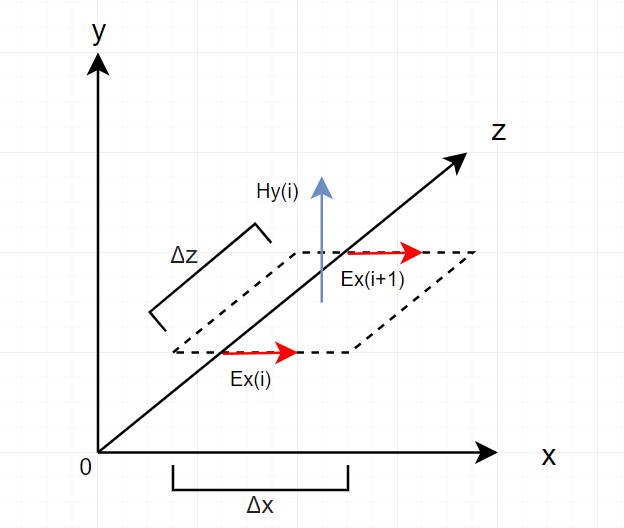
\includegraphics[scale=0.7]{Figures/fdtd1dHcurl}
	\decoRule
	\caption[1D Curl around $H_y$]{A graph showing the one-dimensional curl around the vector $H_y(i)$.}
	\label{fig:fdtd1dHcurl}
\end{figure}

Figure \ref{fig:fdtd1dHcurl} shows the curl around the magnetic vector $H_y(i)$. We can use this curl and plug it in to the original equation \ref{eqn:electricUpdateIntegral}:

\begin{equation}
	\label{eqn:magneticCurl1}
	\oint E \cdot ds = E_x(i) \cdot \Delta x + E_z \cdot \Delta z - E_x(i+1) \cdot \Delta x - E_z \cdot \Delta z
\end{equation}

Since we do not have an Ez vector in the one-dimensional scenario, $Ez \cdot \Delta z = 0$. Therefore we can simplify equation \ref{eqn:magneticCurl1} to:

\begin{equation}
	\label{eqn:magneticCurl2}
	\oint E \cdot ds = E_x(i) \cdot \Delta x - E_x(i+1) \cdot \Delta x
\end{equation}

On the left hand side of equation \ref{eqn:electricUpdateIntegral} we have:

\begin{equation}
	\label{eqn:magneticCurl3}
	\int \mu \cdot H \cdot dA = \mu \int H \cdot dA = \mu \cdot H_y(i) \cdot \Delta y \cdot \Delta z
\end{equation}

By combining \ref{eqn:magneticCurl2} and \ref{eqn:magneticCurl3}, we get:

\begin{equation}
	\label{eqn:magneticCurl4}
	\Delta x(E_x(i) - E_x(i+1)) = -\frac{d}{dt} (\mu \cdot H_y(i) \cdot \Delta y \cdot \Delta z)
\end{equation}

\begin{equation}
	\label{eqn:magneticCurl5}
	E_x(i) - E_x(i+1) = -\mu \cdot \Delta z \cdot \frac{dH_y(i)}{dt}
\end{equation}

We can do the same thing for the curl of the electric vector $E_x$, shown in Figure \ref{fig:fdtd1dEcurl}, as follows (Similar to the previous scenario, $H_z = 0$):

\begin{figure}
	\centering
	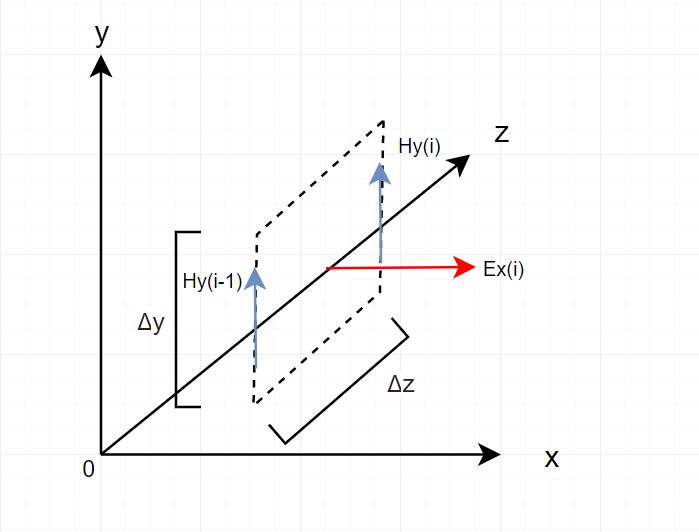
\includegraphics[scale=0.7]{Figures/fdtd1dEcurl}
	\decoRule
	\caption[1D Curl around $E_x$]{A graph showing the one-dimensional curl around the vector $E_x(i)$.}
	\label{fig:fdtd1dEcurl}
\end{figure}

\begin{equation}
	\label{eqn:electricCurl1}
	\oint H \cdot ds = H_y(i) \cdot \Delta y - H_y(i-1) \cdot \Delta y = \Delta y (H_y(i) - H_y(i-1))
\end{equation}

\begin{equation}
	\label{eqn:electricCurl2}
	\iint \epsilon \cdot E \cdot dA = \epsilon \cdot E_x(i) \cdot \Delta z \cdot \Delta y
\end{equation}

Combining \ref{eqn:electricCurl1} and \ref{eqn:electricCurl2}:

\begin{equation}
	\label{eqn:electricCurl3}
	\Delta y (H_y(i) - H_y(i-1)) = \frac{d}{dt} (\epsilon \cdot E_x(i) \cdot \Delta z \cdot \Delta y)
\end{equation}
\begin{equation}
	\label{eqn:electricCurl4}
	H_y(i) - H_y(i-1) = \epsilon  \cdot \Delta z  \cdot \frac{d}{dt} E_x(i)
\end{equation}

With those equations, we can now use the leapfrog time scheme to stagger our components along the time axis (Fig. \ref{fig:fdtd1dLeapfrog}).

\begin{figure}[!h]
	\centering
	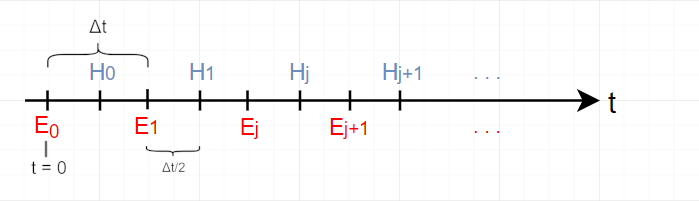
\includegraphics[scale=0.75]{Figures/fdtd1dLeapfrog}
	\decoRule
	\caption[Leapfrog Time Scheme]{Staggering the components along the time axis t using the leapfrog time scheme}
	\label{fig:fdtd1dLeapfrog}
\end{figure}

We will use the following indexing scheme:

\begin{equation}
	\label{eqn:indexingElectric}
	E_{i,j} = E(i \cdot \Delta z , j \cdot \Delta t)
\end{equation}

\begin{equation}
	\label{eqn:indexingMagnetic}
	H_{i,j} = H((i + \frac{1}{2}) \cdot \Delta z , (j + \frac{1}{2}) \cdot \Delta t)
\end{equation}

Using \ref{eqn:indexingElectric} and \ref{eqn:indexingMagnetic} we get the following time derivatives:

\begin{equation}
	\label{eqn:timeDerivativeE}
	\frac{d E_x}{dt} \bigg\rvert_{\underset{z = i \cdot \Delta z}{t=(j + \frac{1}{2})\Delta t}} = \frac{E_{x^{i,j+1}} - E_{x^{i,j}}}{\Delta t}
\end{equation}

\begin{equation}
	\label{eqn:timeDerivativeH}
	\frac{d H_y}{dt} \bigg\rvert_{\underset{z = (i + \frac{1}{2}) \Delta z}{t=j \cdot \Delta t}} = \frac{H_{y^{i,j}} - H_{y^{i,j-1}}}{\Delta t}
\end{equation}

Going back to equation \ref{eqn:magneticCurl5} we get:

\begin{equation}
	\label{eqn:timeDerivativeE2}
	E_x(i \cdot \Delta z) - E_x((i+1) \cdot \Delta z) = -\mu \cdot \Delta z \cdot \frac{d H_y((i+1/2)\Delta z) }{\Delta t}
\end{equation}

Evaluating at $t = j \cdot \Delta t$ gives us:

\begin{equation}
	\label{eqn:timeDerivativeE3}
	E_{x^{i,j}} - E_{x^{i+1,j}} = -\mu \cdot \Delta z \cdot \frac{H_{y^{i,j}} - H_{y^{i,j-1}}}{\Delta t}
\end{equation}

Finally, by solving for ${H_{y^{i,j}}}$ we get our update equation for the magnetic element:
	
\begin{equation}
	\label{eqn:magneticUpdate}
	H_{y^{i,j}} = H_{y^{i,j-1}} - \frac{\Delta t}{\mu \cdot \Delta z}(E_{x^{i,j}} - E_{x^{i+1,j}})
\end{equation}

In a similar way, we can get the update equation for the electric element by starting from the equation \ref{eqn:electricCurl4}. The result is:

\begin{equation}
	\label{eqn:electricUpdate}
	E_{x^{i,j+1}} = E_{x^{i,j}} + \frac{\Delta t}{\epsilon \cdot \Delta z}(H_{y^{i,j}} -  H_{y^{i-1,j}})
\end{equation}

Finally, we are ready to proceed into the code implementation.

%----------------------------------------------------------------------------------------
%	SECTION 2
%----------------------------------------------------------------------------------------

\section{C++ Implementation}

Calculating the update equations is by far the most difficult part of implementing FDTD. However, translating equations into code is not always straightforward. Before we begin the implementation, we need to prepare our coding environment. For this project, the author is using the Eclipse IDE for C++ Development\textsuperscript{\cite{eclipse}}. After creating a new project, we will start off with an empty skeleton that features the \textit{main()} method. Due to not needing any other classes, this is where we will place our code. Before that, we will need to include some packages so that we can use their methods.

\begin{minted}[breaklines,frame=single,fontsize=\footnotesize]{c++}
#define _USE_MATH_DEFINES
	
#include <iostream>
#include <stdio.h>
#include <math.h>
#include <stdlib.h>
#include <cmath>
#include <vector>
#include <string>

using namespace std;
\end{minted}

To shortly explain what each line does:

\begin{itemize}
	\item \textbf{cmath, math.h} - Packages that allow the use of various helpful math related commands and constants. Requires having \space \verb!#define _USE_MATH_DEFINES! set in order for everything to work properly
	\item \textbf{iostream, stdio.h} - Allows for the usage of input and output stream objects and commands. In the 1D implementation, we will print our data to the console by using \verb!cout!
	\item \textbf{stdlib.h} - Provides helpful data types, especially when dealing with vectors
	\item \textbf{vector} - Arrays in C++ are not dynamic. Once populated, they can no longer be modified. That is why for this implementation we need to use vectors.
	\item \textbf{string} - Includes the string datatype. A string is basically an array of characters. Not only can we use this to format our output more easily, it can also be very useful for printing debugging messages.
\end{itemize}

\section{Data Visualization}

\begin{figure}
	\centering
	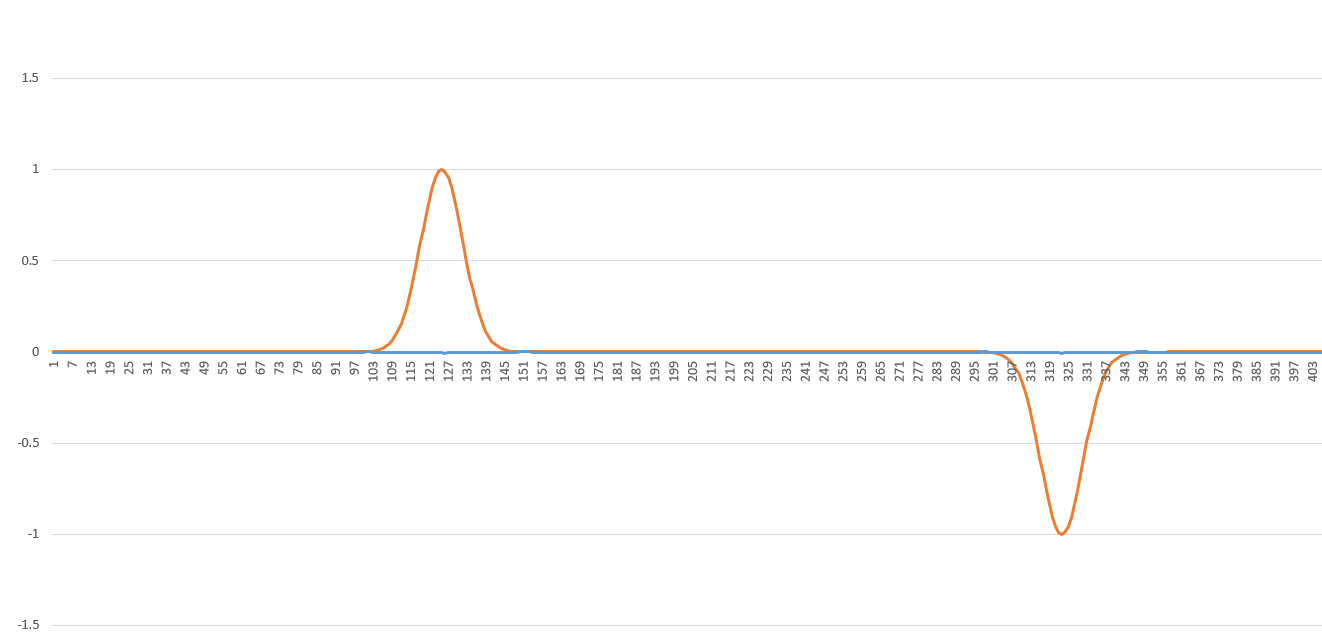
\includegraphics[scale=0.65]{Figures/1DtimeGraph1}
	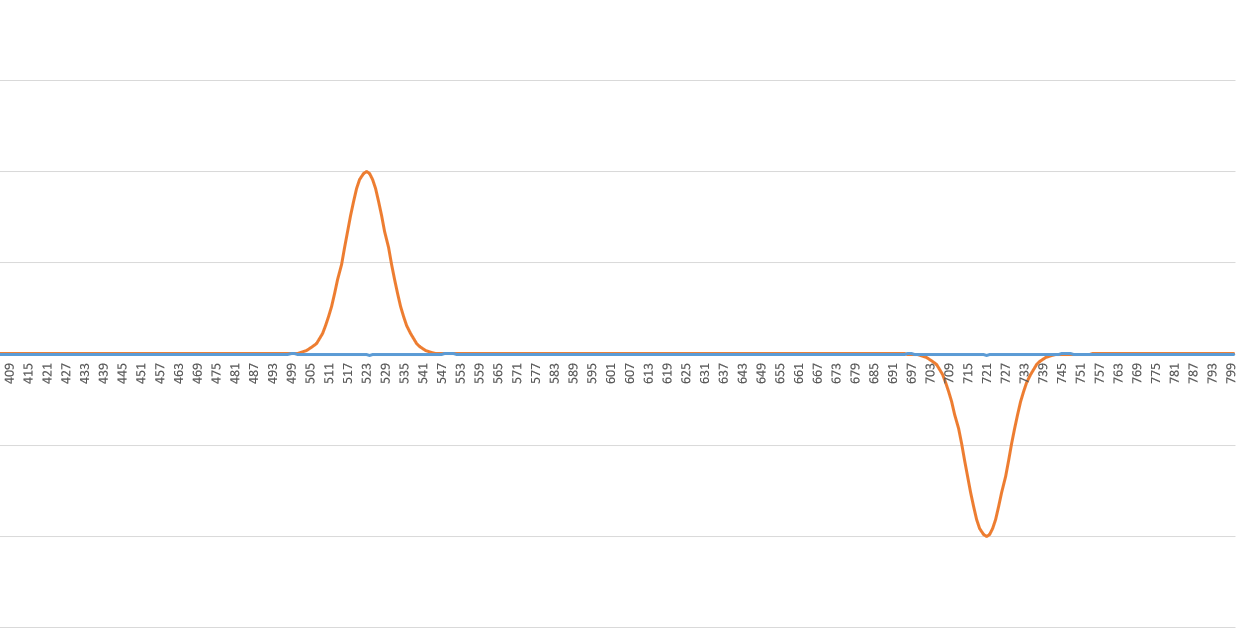
\includegraphics[scale=0.7]{Figures/1DtimeGraph2}
	\decoRule
	\caption[1D Electromagnetic Time Graph]{The time graph of the electromagnetic data generated by our 1D application.}
	\label{fig:emTimeGraph}
\end{figure}

\begin{figure}
	\centering
	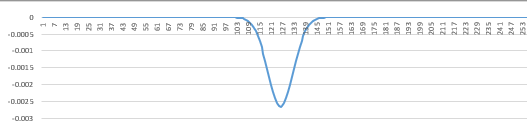
\includegraphics{Figures/1DmagneticTimeSnippet}
	\decoRule
	\caption[1D Magnetic Time Snippet]{A snippet of the time graph shown in Figure \ref{fig:emTimeGraph} zoomed in}
	\label{fig:mTimeSnippet}
\end{figure}